\documentclass{article}

\usepackage[utf8]{inputenc}
\usepackage[T1]{fontenc}
\usepackage{lmodern}
\usepackage[ngerman]{babel}
\usepackage{amsmath}
\usepackage{amsfonts}
\usepackage{graphicx}
\usepackage{hyperref}
\usepackage{media9}
\usepackage{multimedia}
\usepackage{ marvosym }
\usepackage{enumitem,xcolor}

\title{Zum Rotationsspiel}
\author{Lars Müller}
\date{20. - 31. Januar 2020}
\begin{document}

\maketitle
\tableofcontents
\section{Einleitung}

Das Rotationsspiel ist ein einfaches Einzelspielerspiel.

\subsection{Anleitung}

\subsubsection{Aufbau}

\begin{figure}
    \centering
    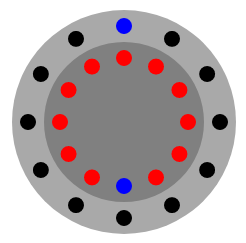
\includegraphics[width=200pt]{darstellung.png}
    \caption{Aufbau}
    \label{fig:darstellung}
\end{figure}

Erklärung zu \ref{fig:darstellung} :

\begin{itemize}
    \item[\textcolor{lightgray}{\textbullet}] Hellgraue Scheibe: Spielbrett
    \item[\textcolor{gray}{\textbullet}] Dunkelgraue Scheibe: Drehbare Scheibe    \item[\textcolor{black}{\textbullet}] Schwarze Punkte: Freie Steckplätze
    \item[\textcolor{blue}{\textbullet}] Blaue Punkte: Feste Pins
    \item[\textcolor{red}{\textbullet}] Rote Punkte: Zu verschiebende Pins
\end{itemize}

\subsubsection{Spielablauf}

Zu Beginn des Spiels muss die Scheibe so ausgerichtet sein, dass die blauen Pins senkrecht zueinander stehen.
Der rote Pin, der unter dem blauen Pin des Bretts liegt, muss pro Zug verschoben werden. 
Dazu darf man ihn einen beliebigen freien Steckplatz des Brettes drehen, in den dieser dann gesteckt wird.
Dies wiederholt man solange, bis kein roter Pin mehr unter dem blauen Pin des Brettes liegt.

Ziel des Spiels ist es, am Ende nur noch den blauen Pin auf der Scheibe, und alle roten Pins auf dem Brett zu haben.
Sind noch welche auf der Scheibe übrig, verliert man.

Anmerkung: Im Original ist das Brett quadratisch und die blauen Pins sind Pfeile.

\subsubsection{Varianten}

\begin{figure}
    \centering
    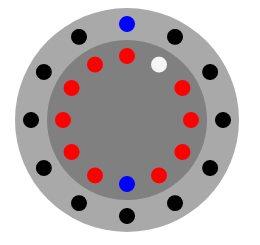
\includegraphics[width=200pt]{darstellung_weiss.png}
    \caption{Mit weißem Pin}
    \label{fig:darstellung_weiss}
\end{figure}

Dem Spiel kann ein weißer Pin hinzugefügt werden, der nur als letzter Pin gedreht werden darf. Müsste er vorher gedreht werden, verliert man.

\begin{figure}
    \centering
    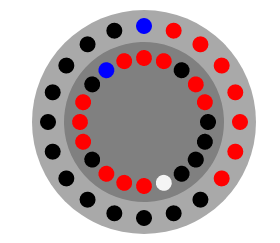
\includegraphics[width=200pt]{darstellung_20.png}
    \caption{Mit weißem Pin und 20 Steckplätzen}
    \label{fig:darstellung_20}
\end{figure}

Weiter kann auch mit mehr Pins und einem entsprechend größeren Brett gespielt werden.

Es wäre auch denkbar, andere Startsituationen zu betrachten, bei denen die blauen Pins in einem anderen Winkel zueinander stünden.

%% \href{run:/usr/local/bin/mplayer -fs beispiel_erfolgreich.mkv}{siehe Beispiel}

\section{Formalisierungsvorschlag}
Zunächst einige Definitionen:
$
n := \text{Anzahl Steckplätze} \\
B := \{b \in \mathbb{B}^n \text { | } b_1 = 1\} \text{ Menge aller möglichen Bretter b mit } b_m := \text{m-ter Steckplatz belegt}\\
S := \{s \in \mathbb{B}^n \text { | } s_{n/2} = 1\} \text{ Menge aller möglichen Scheiben s mit } s_m := \text{m-ter Steckplatz belegt}\\
z := (b, s) \text { Spielzustand}, z_s := Startzustand \\
l := \{m \in {(\mathbb{N} \setminus 0)}^n \text{ | } m_i \leq n \}\text{ Lösungen }
$
Rotationen lassen sich als Index-Shift des Drehscheiben-Tupels darstellen:
Weiter gilt, dass jede Rechtsrotation um g Grad einer Linksrotation um 360-g Grad gleicht.
Außerdem gilt für jede Rotation um g Grad, dass diese einer Rotation um g mod 360 entspricht
$
r\colon S, \mathbb{N} \to S \\
s, k \mapsto r(s, k) = d \text{ mit } d_n = s_{(n+k) \mod n}
$
Spielzüge entsprechend als Funktion:
$
t\colon Z, \mathbb{N} \to Z \\
z, k \mapsto t(z, k) = (o, u=r(s, k)) \text{ mit } o_k = 1 \text{ und } u_k = 0
$
Ein Spielzustand ist gewonnen, genau dann wenn die Scheibe leer ist (abgesehen vom festen)
$
\text{z gewonnen } \Leftrightarrow \forall l \leq n \land l \neq n/2 \colon s_n = 0 \\
$
Entsprechend:
$
t'\colon Z, \mathbb{N}^n \to Z \\
    z, k' \mapsto t'(z, k) =  \begin{cases} 
        t'(t(z, k'_{|k'|}), (k'_1, k'_2, ..., k'_{|k'|-1})) & |k'| > 0 \\
        z & |k'| = 0
    \end{cases}
    \\
\text{l Lösung } \Leftrightarrow t'(z_s, l) gewonnen \\
$
Feststellungen: Mit jedem Zug gibt es eine Möglichkeit weniger, die Scheibe zu drehen.
Somit haben wir als obere Abschätzung $(n-1)!$ - Für unser herkömmliches Spiel mit n=11 also etwa 4 Millionen Möglichkeiten, ein leichtes für eine Brute-Force. \\
\subsection{Endlicher Automat}
\text{Alternativ: endlicher Automat mit Spielzuständen und Endzuständen = gewonnene Zustände}
Die Menge aller Lösungen wäre dann die Sprache des Automaten.
$
Q = Z \\
s = z_s \\
\Sigma = \{a \in \mathbb{N} | a \in [1, n-1]\} \\
F = {z \in Z | \text{z gewonnen}} \\
\delta = t
$

\subsection{Strategien}

Wir dürfen nicht so drehen, das Insgesamtdrehung $d = n/2$, denn dann ist der blaue Pin oben.
Außerdem dürfen wir auch nicht so drehen, dass $d_m \equiv d_m \mod l \;\land\; m \neq l$.

\subsection{Position des blauen Pins}
Einfach anzugeben durch $\sum_{i=1}^{n-1} i \mod n = \lfloor\frac{n}{2}\rfloor + \frac{(n-1) \cdot n}{2} \mod n = 0\\$
$\Rightarrow \text{ Blauer Pin immer oben }$

\section{Lösungsalgorithmen}

\subsection{Brute-Force}
Aufgrund der stark steigenden Möglichkeiten kommt eine Brute-Force, die alle Lösungen findet, nur für relativ kleine n (~ < 20) infrage.
Auch andere Algorithmen würden dabei komplex werden. Ein Bestimmen der bloßen Anzahl allerdings könnte durchaus performant sein.
Will man jedoch nur Eine finden, ist die Brute-Force auch für größere n (etwa n=100) noch performant.

\begin{figure}
    \centering
    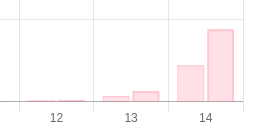
\includegraphics[width=200pt]{graph.png}
    \caption{Steigende Komplexität}
    \label{fig:graph}
\end{figure}

Wie in \ref{fig:graph} zu sehen ist, scheinen Komplexität (der Brute-Force) und Anzahl der Lösungen exponentiell anzusteigen.

\subsection{Füllen}
Für $n = 2^k$ Zweierpotenzen kann man einfach ``füllen'' (jedes Mal eins weiter drehen), d. h. $l \in \mathbb{L}, l = (1, 2, ..., n-1) $

Etwa für n=16: $l_1 \in \mathbb{L}, l_1 = (1, 2, 3, ..., 15)$ oder allgemein $n=2^k \Rightarrow l_1 = (1, 2, ..., n-1)$ 
Dass so das Brett ``der Reihe nach'' gefüllt wird, ist klar. Es bleibt zu zeigen, wieso immer ein roter Pin unter dem Blauen landet.
\\
Damit unser Verfahren scheitert, muss:\\
\begin{enumerate}
    \item Auf eine bereits ``geleerte'' Position gedreht werden
    \item Auf den blauen Pin (der Scheibe) gedreht werden
\end{enumerate}
Für $n=2$ ist nur eine Drehung - um 1 - möglich. Wir betrachten also $n > 2$.\\
Zu 1: Widerspruchsbeweis\\
$
d_y := \frac{y \cdot (y-1)}{2} \mod n \text{ (Insgesamtdrehung) } \\
\text{Zu zeigen: }d_1 \neq d_2 \neq ... \neq d_{n-1} \\
y, y' \in \mathbb{N}, [1, n-1] \land y \neq y'
\Rightarrow y' = y + x \land x \neq 0 \\
d_y = d_{y'} \\
\Leftrightarrow \frac{y \cdot (y-1)}{2} \mod n = \frac{y' \cdot (y'-1)}{2} \mod n \\
\Leftrightarrow \frac{y \cdot (y-1)}{2} \equiv \frac{y' \cdot (y'-1)}{2} \mod n \\
\Leftrightarrow y \cdot (y-1) \equiv y' \cdot (y'-1) \mod \frac{n}{2} \\
\Leftrightarrow y \cdot (y-1) \equiv (y+d) \cdot (y+d-1) \mod \frac{n}{2} \\
\Leftrightarrow y \cdot (y-1) \equiv y^2 + 2yd - y + d^2 - d \mod \frac{n}{2} \\
\Leftrightarrow y^2 - y \equiv y^2 - y + 2yd +d^2 - d \mod \frac{n}{2} \\
\Leftrightarrow \frac{n}{2}\; | \;(y^2 - y + 2yd +d^2 - d) - (y^2 - y) \\
\Leftrightarrow \frac{n}{2}\; | \;2yd + d^2 - d \\
\Leftrightarrow \frac{n}{2}\; | \;d \cdot (2y + d - 1) \\
\Leftrightarrow 2^{k-1}\; | \;d \cdot (2y + d - 1) \\
\Rightarrow d \cdot (2y + d - 1) = 2^l \\
\text{1. Fallunterscheidung:} \\
d = 1 \Rightarrow 2^{k-1}\; | \;2y\\
\text{1. 1. Fallunterscheidung:} \\
y = 1 \Rightarrow 0 \equiv 1 \mod \frac{n}{2} \Rightarrow \text{ \Lightning \; da } \frac{n}{2} > 1\\
y = 2^o \Rightarrow \text{ \Lightning \; da } 2^{k-1} < y < 2^k \text{ ($y$ liegt zwischen zwei ``benachbarten'' Zweierpotenzen $\Rightarrow$ kann selbst keine sein)}\\
d = 2^m \Rightarrow 2^l = 2^m \cdot (2y + 2^m - 1) = 2^m (2 \cdot (y + 2^{m-1}) - 1)) \; aber \; 2 \cdot n - 1 \not| \; 2 \: \text{\Lightning}
\\ \text{\large{\Lightning}} \Box
$
\\Weiter können wir folgern, dass nicht vor Ende auf den blauen Pin gedreht werden kann: \\
Blauer Pin am Ende auf Position 0 $\land$ kein Pin zwei Mal an Position 0 $\Rightarrow$ Blauer Pin nicht vor Ende auf Position 0. 
\\Und schließlich:\\
Kein Pin zwei Mal an Position 0 $\land$ Auf blauen Pin wird erst am Ende gedreht $\Rightarrow$ Alle Drehungen können durchgeführt werden $\Rightarrow$ Lösung! 

\subsubsection{Weißer Pin}
Spielt man mit dem weißen Pin, muss dieser an der Stelle 
$p_w = (1 + 2 + ... + n-1 = \sum_{i=1}^{n-1} = \frac{n \cdot (n-1)}{2}) \mod n$ stehen

\subsection{Gruppenvergleich}
\begin{itemize}
    \item Funktioniert für $n=12$ (aber sonst nur für wenige Andere)
    \item Findet nur eine Lösung
    \item Einprägsam
\end{itemize}

Die Gruppen an Pins auf der Scheibe müssen den Gruppen an Löchern auf dem Brett entsprechen und vice-versa.

\subsection{Permutieren}

Hierbei nehmen wir alle nötigen Drehungen $d = (1, ..., n-1)$ und suchen eine Permutation, für die gilt:

$
\Sigma_{d_1}^{d_{k}} \equiv \Sigma_{d_1}^{d_{l}} \mod n \Rightarrow k = l \\
\land \Sigma_{d_1}^{d_{k}} \equiv \frac{n}{2} \mod n \Rightarrow k = n-1
$

In der Implementation wird eine beliebige Permutation so lange zum ``Besseren'' permutiert (optimiert, Problemreduktion), bis es keine Probleme mehr gibt.

\subsection{Leeren}

Beim ``Leeren'' wird die Scheibe mit abwechselnden Links/-Rechtsdrehungen systematisch geleert.\\\\
$
n := 2k, k \in \mathbb{N} \\
d = (1, n-2, 3, n-4, ..., n-1, 2) \\
$
\\\\
Wieso das Brett am Ende voll sein muss, ist klar:
$d$ ist eine Permutation von $(1, 2, ..., n-1)$ - auf jeden freien Steckplatz des Brettes wird einmal gedreht.
\\\\
Sei $g(y)$ die geleerte Position im $y$-ten Schritt:\\
$
R := \{y \in \mathbb{N} \; | \; y \in [1, n-1]\}\\
G := \{x \in \mathbb{N} \; | \; x \in [1, n-1]\}\\
g\colon R \to G\\
y \mapsto g(y) = \begin{cases}
\frac{y(n-1)}{2} \mod n & \text{$y$ gerade} \\
(\frac{(y-1)(n-1)}{2} + y) \mod n & \text{$y$ ungerade}
\end{cases}\\
g^{-1}\colon G \to R\\
x \mapsto g^{-1}(x) = \begin{cases}
    2 \cdot (n-y) & y > \frac{n}{2} \\
    2y - 1 & y \leq \frac{n}{2}
    \end{cases}\\
$
Werte von $g(y)$ für $n=12$:
\begin{center}
    \begin{tabular}{| c | c | c | c | c | c | c | c | c | c | c | c |}
    \hline
     $y$ & 1 & 2 & 3 & 4 & 5 & 6 & 7 & 8 & 9 & 10 & 11 \\
     \hline
     $g(y)$ & 1 & 11 & 2 & 10 & 3 & 9 & 4 & 8 & 5 & 7 & 6 \\
     \hline
    \end{tabular}
\end{center}
$
\text{Zu zeigen: } g^{-1}(g(y)) = y \Rightarrow\text{ g bijektiv }\Rightarrow g(1) \neq g(2) \neq ... \neq g(n-1)
\\\text{Fallunterscheidung:}
\\\text{$y$ gerade} \Rightarrow y = 2k,\, g(y) = \frac{y(n-1)}{2} \mod n\\\\
\frac{y(n-1)}{2} \mod n = \frac{2k(n-1)}{2} \mod n = kn-k \mod n = \boxed{n - k > \frac{n}{2}} - \text{ klar, da $k < \frac{n}{2}$ gilt}\\
\Rightarrow g^{-1}(\frac{y(n-1)}{2} \mod n) = 2 \cdot (n-((kn - k) \mod n)) = 2 \cdot (n-(n-k)) = 2k = y \\
\\\text{$y$ ungerade} \Rightarrow y = 2k + 1,\, g(y) = (\frac{(y-1)(n-1)}{2} + y) \mod n\\\\
(\frac{y(n-1)}{2} + y) \mod n = \frac{(y+1)(n-1)+2y}{2} \mod n = \frac{(2k+1)(n-1)}{2} \mod n
= \frac{(2k+1)(n-1)+2k+1}{2} \mod n = \frac{2kn-2k+n-1+2k+1}{2} \mod n = \frac{2kn+2 \cdot \frac{n}{2}}{2} \mod n
= kn+\frac{n}{2} \mod n = \boxed{\frac{n}{2} \leq \frac{n}{2}} \\
\Rightarrow g^{-1}((\frac{(y-1)(n-1)}{2} + y) \mod n) = 2 \cdot ((\frac{(y-1)(n-1)}{2} + y) \mod n) - 1 \\
= 2 \cdot ((\frac{(y-1)(n-1)}{2} + y) \mod n) - 1 = 2 \cdot ((\frac{(2k + 1 -1)(n-1)}{2} + 2k + 1) \mod n) - 1 = 2 \cdot ((k(n-1) + 2k + 1) \mod n) - 1 \\
= 2 \cdot ((k(n-1) + 2k + 1) \mod n) - 1 = 2 \cdot ((kn - k + 2k + 1) \mod n) - 1 = 2 \cdot (k + 1) - 1 = 2k + 2 - 1 = 2k + 1 = y
\\\Box\\
$
Analog zu ``Füllen'' können wir folgern, dass diese Strategie eine Lösung darstellt - auf keine Position der Scheibe wird zweimal gedreht und der blaue Pin ist, wie schon gezeigt, am Ende oben.

\subsubsection{Weißer Pin}
Spielt man mit dem weißen Pin, muss dieser an der Stelle 
$p_w = g(n-1) = (\frac{(n-2)(n-1)}{2} + n - 1) \mod n$ stehen.\\
So ist beim herkömmlichen Spiel mit $n=12$ die Position $p_w = g(11) = 66 \mod 12 = 6$ - der weiße Pin muss also - bei Anwenden der Strategie - rechts vom Blauen stehen. 
Wendet man die Strategie mit Links- und Rechtsdrehungen vertauscht an, muss er links vom blauen Pin positioniert sein.
\end{document}